\newpage
\setcounter{subsection}{0}
\section{ESTADO DEL ARTE}

La infraestructura subyacente a la emisión y distribución de boletería digital experimenta en la actualidad
una transición insoslayable. Dicho paradigma migratorio obedece a la imperativa necesidad técnica de mitigar
el fraude sistémico, desincentivar el arbitraje especulativo y reestructurar la confianza del consumidor
final. El presente capítulo disecciona de manera analítica los modelos operativos convencionales
(arquitecturas Web2), escudriña el surgimiento de las alternativas descentralizadas sustentadas en registros
distribuidos (Web3) y argumenta, desde una base empírica y conceptual, la pertinencia arquitectónica del
ecosistema híbrido (Web2.5) desarrollado en esta investigación.

\subsection{Sistemas Centralizados y Asimetría de Información (Web2)}

Históricamente, los canales de distribución primaria y los mercados secundarios de reventa han sido
monopolizados por consorcios tecnológicos que fungen como custodios absolutos tanto de la topología de la
información como de la conciliación financiera. 

\subsubsection{Estructuras de mercado primario (Ticketmaster, Eventbrite)}

Los conglomerados líderes del sector, tales como Ticketmaster \cite{ticketmaster2024} y Eventbrite, sostienen
sus operaciones sobre arquitecturas de microservicios o sistemas monolíticos donde el activo —el boleto— no
es más que un registro inerte dentro de una base de datos relacional privada (generalmente clústeres
PostgreSQL o MySQL) vinculada unívocamente a las credenciales de un usuario. En un esfuerzo por neutralizar
la proliferación de archivos PDF falsificados, estas entidades implementaron esquemas criptográficos
superficiales, ejemplificados en la rotación temporal de códigos QR dinámicos (como la patente
\textit{SafeTix}).

Pese a que tales contramedidas robustecen el control de acceso perimetral en la puerta del recinto, el modelo
adolece de profundas fisuras estructurales en lo referente a la trazabilidad de la propiedad:
\begin{enumerate}
    \item \textbf{Hermetismo de datos (Silos):} La validación de la legitimidad del título de ingreso queda
restringida a las fronteras del ecosistema cerrado del proveedor, impidiendo la verificación externa o la
auditoría pública.
    \item \textbf{Fricción en la interoperabilidad:} Al carecer de un canal oficial seguro para ceder el
activo fuera del control de la entidad matriz, los usuarios recurren a métodos analógicos o cesión de
credenciales, lo cual reintroduce el riesgo de duplicación paralela o \textit{double-spending} en el mercado
gris.
\end{enumerate}

\subsubsection{Arbitraje desregulado en la reventa (StubHub, Viagogo)}

Las infraestructuras concebidas para absorber la demanda secundaria, ejemplificadas por StubHub \cite{stubhub2024}, operan primordialmente como agentes fiduciarios o pasarelas de \textit{escrow}. Bajo este esquema, el capital del adquirente se pignora hasta la culminación del evento, procurando certificar empíricamente la validez del acceso. Si bien este mecanismo salvaguarda el patrimonio financiero del comprador ante estafas burdas, carece de la capacidad técnica para invalidar preventivamente un boleto que haya sido comercializado simultáneamente en múltiples foros. Consecuentemente, el usuario malicioso conserva la posibilidad de defraudar a varios actores, mientras la plataforma extrae rentabilidades operativas que frecuentemente oscilan entre el 15\,\% y el 30\,\% \cite{scand2023ticketing}, un modelo que inherentemente incentiva y capitaliza la especulación.

\subsection{Alternativas Descentralizadas y la Promesa de los NFTs (Web3)}

La irrupción de la tecnología de cadenas de bloques catalizó el modelo de \textit{NFT Ticketing}. Mediante
este diseño, cada entrada se materializa como un token no fungible en una red pública, lo que provee, por
mandato criptográfico, la anhelada escasez digital y una cronología inmutable sobre el historial de
transferencias \cite{ieee2023nft}.

\subsubsection{Protocolos de Infraestructura B2B (OPEN Ticketing Ecosystem)}

El ecosistema OPEN, previamente consolidado bajo la denominación GET Protocol \cite{getprotocol2024},
constituye el marco de referencia más maduro para la emisión programable on-chain. Dicha infraestructura
opera como una capa de marca blanca que habilita a las tiqueteras convencionales a acuñar activos sobre redes
compatibles con la Máquina Virtual de Ethereum (EVM), con particular énfasis en cadenas laterales como
Polygon.

La principal aportación empírica de estas arquitecturas reside en la capacidad de los organizadores para
incrustar lógicas de negocio directamente en el código del activo. Esto facilita la imposición de techos de
precios algorítmicos y la ejecución determinista de regalías (\textit{royalties}) en transacciones
secundarias \cite{scand2023ticketing}. No obstante, la dependencia de entornos EVM conlleva vulnerabilidades
estructurales: la volatilidad estocástica de los costos de transacción (\textit{gas fees}) frente a picos de
congestión y los riesgos derivados de mantener metadatos almacenados de forma paralela (\textit{off-chain}),
lo cual puede ser explotado si los oráculos de sincronización son comprometidos \cite{ieee2023nft}.

\subsubsection{Plataformas de Audiencia y Riesgos Inherentes (YellowHeart, SeatlabNFT)}

En contraste, soluciones orientadas hacia el consumidor final como SeatlabNFT \cite{seatlab2024} y
YellowHeart \cite{yellowheart2024} apostaron por expandir la utilidad del boleto más allá del acceso físico,
transformándolo en un vector de fidelización (\textit{engagement}) mediante beneficios perpetuos y
recompensas comunitarias. 

Sin embargo, el consenso académico e industrial advierte que la adopción de plataformas Web3 puras impone
barreras sistémicas severas. La responsabilidad de gestionar llaves criptográficas privadas transfiere una
carga cognitiva inasumible para el usuario promedio \cite{wolfandco2023}. Aunado a ello, la propia
inmutabilidad de los contratos inteligentes dicta que cualquier defecto en la compilación del código puede
resultar en pérdidas irrevocables, y el usuario no técnico queda expuesto a ataques de ingeniería social o
\textit{phishing} sofisticado frente a los cuales las arquitecturas descentralizadas no ofrecen mecanismos
centralizados de restitución \cite{wolfandco2023}.

\subsubsection{Iniciativas sobre redes de alto rendimiento (Solana y Flow)}

El espacio de tokenización de boletería no se circunscribe al ecosistema compatible con la Máquina Virtual de
Ethereum (EVM). Diversos actores de la industria han experimentado con redes de capa base concebidas
específicamente para maximizar el rendimiento transaccional y reducir los costos por operación, lo que
introduce parámetros de comparación distintos a los de las plataformas previamente analizadas.

El caso más visible sobre la red \textbf{Solana} corresponde a la \textit{Coachella Keys Collection}, una
emisión lanzada en 2022 por el festival Coachella que tokenizó pases vitalicios y artículos coleccionables
como NFTs sobre dicha cadena, apoyándose en la infraestructura de mercado de FTX \cite{coachella2022}. Solana
sustituye el costoso consenso por cómputo de las redes PoW por una combinación de \textit{Proof of History}
(PoH) ---un reloj criptográfico verificable que ordena los eventos--- y \textit{Proof of Stake} bajo el
protocolo Tower BFT, lo que le permite anunciar capacidades teóricas de hasta $65\,000$\,TPS con comisiones
del orden de fracciones de centavo de dólar \cite{solana2024}. No obstante, este diseño orientado a la
maximización del rendimiento ha mostrado una tensión estructural con la disponibilidad: la red ha
experimentado múltiples interrupciones totales (\textit{full outages}) documentadas entre 2021 y 2024,
durante las cuales el procesamiento de transacciones se detuvo por completo durante varias horas
\cite{helius2024solana}. Adicionalmente, el desplome de FTX a finales de 2022 ilustró el riesgo de anclar la
experiencia de un activo descentralizado a un custodio o un mercado centralizado, dado que la negociabilidad
y la visualización de los NFTs de Coachella quedaron comprometidas tras la quiebra de la plataforma.

En contraste con la apuesta por el rendimiento puro, \textbf{Ticketmaster} ---el actor dominante del mercado
primario--- habilitó en 2022 la emisión de NFTs ``token-gated'' sobre la red \textbf{Flow} de Dapper Labs
\cite{ticketmasterflow2022}, una cadena con arquitectura multi-rol diseñada para aplicaciones de consumo
masivo y coleccionables digitales \cite{flow2024}. Este movimiento es significativo porque evidencia que
incluso los conglomerados Web2 reconocen el valor de la trazabilidad on-chain; sin embargo, su
implementación se limita a la dimensión de \textit{engagement} (beneficios y coleccionables) y no aborda la
liquidación financiera atómica del mercado secundario, que permanece dentro de los rieles fiduciarios
tradicionales de la plataforma.

El contraste entre estas aproximaciones revela que la elección de la red base no es un detalle de
implementación, sino una decisión arquitectónica con consecuencias directas sobre la disponibilidad, el
costo y la finalidad del sistema. Un modelo de boletería que privilegie la integridad del acceso al evento
no puede tolerar las interrupciones totales observadas en redes optimizadas exclusivamente para el
rendimiento, lo que motiva el análisis comparativo de redes de capa base que se presenta más adelante.

\subsection{Posicionamiento Arquitectónico y Análisis Comparativo}

El estado del arte revela una polarización ostensible: por un lado, la fluidez operativa de la Web2 que
sacrifica la transparencia y fomenta el rentismo; por el otro, el rigor matemático de la Web3 que impone
altos umbrales de fricción cognitiva y exposición a vectores de ataque no convencionales. El presente
desarrollo tecnológico, denominado \textit{SecureTicket}, se ancla deliberadamente en la intersección de
ambos paradigmas, estructurando una topología Web2.5.

La Figura~\ref{fig:espectro-arquitecturas} ilustra de manera esquemática este espectro metodológico,
demarcando el posicionamiento estratégico de los modelos previamente escrutados.

\begin{figure}[H]
\centering
\vspace{0.5cm}
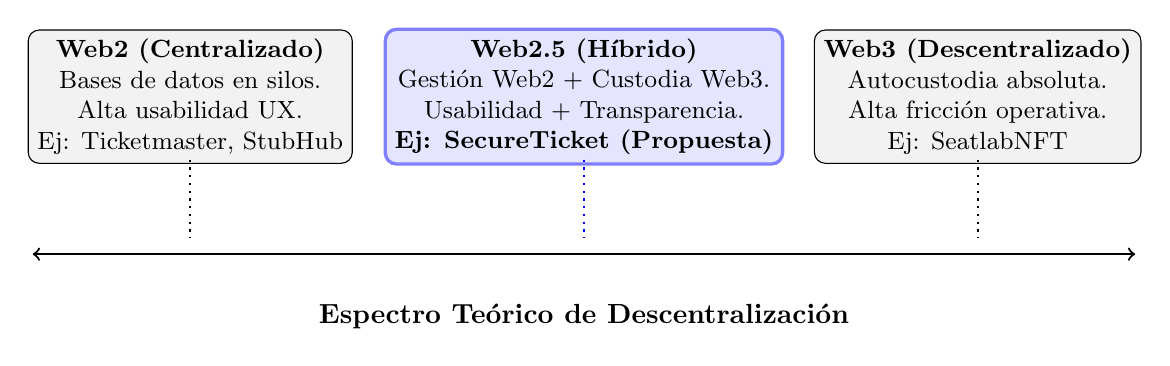
\begin{tikzpicture}[
    box/.style={draw, rounded corners, minimum width=4cm, minimum height=1.5cm, align=center, font=\small},
    arrow/.style={thick, ->, >=stealth}
]

% Eje horizontal
\draw[thick, <->] (0,0) -- (14,0) node[midway, below=0.5cm] {\textbf{Espectro Teórico de Descentralización}};

% Cajas
\node[box, fill=gray!10] (web2) at (2, 2) {\textbf{Web2 (Centralizado)}\\Bases de datos en silos.\\Alta
usabilidad UX.\\Ej: Ticketmaster, StubHub};

\node[box, fill=blue!10, draw=blue!50, very thick] (web25) at (7, 2) {\textbf{Web2.5 (Híbrido)}\\Gestión Web2
+ Custodia Web3.\\Usabilidad + Transparencia.\\\textbf{Ej: SecureTicket (Propuesta)}};

\node[box, fill=gray!10] (web3) at (12, 2) {\textbf{Web3 (Descentralizado)}\\Autocustodia absoluta.\\Alta
fricción operativa.\\Ej: SeatlabNFT};

% Líneas conectivas
\draw[dotted, thick] (2, 1.2) -- (2, 0.2);
\draw[dotted, thick, blue] (7, 1.2) -- (7, 0.2);
\draw[dotted, thick] (12, 1.2) -- (12, 0.2);

\end{tikzpicture}
\vspace{0.5cm}
\caption{Diagrama conceptual: Posicionamiento del modelo híbrido Web2.5 propuesto en contraste con los
axiomas operativos de la industria actual.}
\label{fig:espectro-arquitecturas}
\end{figure}

Con el propósito de sistematizar los contrastes técnicos entre las aproximaciones estudiadas, la
Tabla~\ref{tab:comparativa-estado-arte} consolida la evaluación de cada modelo frente a las vulnerabilidades
críticas del sector: proliferación de duplicados, distorsiones de precio, fricción transaccional y
resiliencia de la experiencia del usuario.

\begin{table}[H]
\centering
\small
\renewcommand{\arraystretch}{1.3}
\definecolor{rowgray}{gray}{0.96}
\caption{Matriz comparativa de atributos arquitectónicos en plataformas de boletería digital.}
\label{tab:comparativa-estado-arte}
\begin{tabularx}{\textwidth}{>{\raggedright\arraybackslash}p{3.5cm} >{\raggedright\arraybackslash}p{3.8cm}
>{\raggedright\arraybackslash}p{3.8cm} >{\raggedright\arraybackslash}X}
\toprule
\rowcolor{rowgray}
\textbf{Atributo Evaluado} & \textbf{Sistemas Web2 (ej. Ticketmaster)} & \textbf{Redes Web3 Puras (ej.
SeatlabNFT)} & \textbf{Modelo Híbrido Web2.5 (Propuesta Actual)} \\
\midrule
\textbf{Soporte de la verdad} & Repositorio central, opaco al escrutinio público. & Ledger criptográfico de
estado global (EVM). & Ledger criptográfico (Stellar) con proyección relacional indexada. \\
\rowcolor{rowgray}
\textbf{Resolución de fraude} & Inoperante en reventas no oficiales (QR clonables). & Erradicado mediante la
unicidad del token no fungible. & Erradicado mediante la semántica atómica \textit{burn/remint} de Soroban. \\
\textbf{Políticas de precios} & Limitación incipiente, sujeta a deducciones arbitrarias. & Restricciones
codificadas de forma inmutable en el contrato. & Topes de especulación inyectados dinámicamente desde el
contrato fábrica. \\
\rowcolor{rowgray}
\textbf{Liquidación financiera} & Retardada, sujeta a ciclos bancarios (72--120h). & Ejecución instantánea en
la capa base mediante criptoactivos. & Ejecución atómica y determinista utilizando dólares digitales (USDC).
\\
\textbf{Fricción de adopción} & Mínima (dependencia de correos y contraseñas). & Severa (necesidad de
custodiar semillas y sufragar \textit{gas}). & Mitigada (autorización mediante \textit{signatures} delegadas,
sin costo para el usuario). \\
\bottomrule
\end{tabularx}
\end{table}

A la luz de esta matriz, el ensamble Web2.5 orquestado sobre el protocolo Stellar emerge como el compromiso
técnico óptimo. Conserva la elasticidad interactiva a la que está habituado el consumidor tradicional,
mientras exilia el fraude P2P y la especulación desmedida delegando la lógica de propiedad y compensación al
motor determinista de la cadena de bloques.

\subsection{Comparativa de redes de capa base para la tokenización de boletos}

La sección anterior contrastó modelos de plataforma (Web2, Web3 y Web2.5); sin embargo, dentro del
paradigma descentralizado la red de capa base (L1) sobre la que se acuñan los activos determina atributos
críticos para un sistema de boletería: el costo por operación, la velocidad de finalidad, la capacidad de
procesamiento y, de forma frecuentemente subestimada, la disponibilidad del servicio. Las plataformas
analizadas se distribuyen sobre redes heterogéneas: GET Protocol y YellowHeart operan sobre entornos
EVM (Ethereum y la cadena lateral Polygon), Coachella experimentó sobre Solana y Ticketmaster sobre Flow.
La Tabla~\ref{tab:comparativa-redes} sistematiza los parámetros técnicos de estas redes frente a la
propuesta de este trabajo sobre Stellar.

\begin{table}[H]
\centering
\small
\renewcommand{\arraystretch}{1.3}
\definecolor{rowgray}{gray}{0.96}
\caption{Comparativa de redes de capa base para la emisión de boletos tokenizados.}
\label{tab:comparativa-redes}
\begin{tabularx}{\textwidth}{>{\raggedright\arraybackslash}p{2.4cm} >{\raggedright\arraybackslash}p{2.7cm}
>{\raggedright\arraybackslash}p{2.0cm} >{\raggedright\arraybackslash}p{2.2cm}
>{\raggedright\arraybackslash}X}
\toprule
\rowcolor{rowgray}
\textbf{Red} & \textbf{Consenso} & \textbf{TPS nominal} & \textbf{Costo aprox. por tx} & \textbf{Rasgo
distintivo} \\
\midrule
Ethereum 1.0 & PoW (histórico) / PoS & 15--30 & USD 5--50 (\textit{gas} volátil) & Congestión y costo
impredecible en picos. \\
\rowcolor{rowgray}
Polygon (PoS) & PoS, cadena lateral EVM & $\approx$\,7\,000 & $<$ USD 0{,}01 & Bajo costo, pero depende de
\textit{checkpoints} anclados en Ethereum. \\
Solana & PoH + PoS (Tower BFT) & hasta 65\,000 (menor en la práctica) & $\approx$\,USD 0{,}00025 & Altísimo
rendimiento, pero con historial de caídas totales de red \cite{helius2024solana}. \\
\rowcolor{rowgray}
Flow & PoS multi-rol & miles & bajo & Orientada a NFT de consumo y coleccionables (Dapper Labs). \\
\textbf{Stellar (propuesta)} & SCP (FBA) & 1\,000--3\,000 & $\approx$\,0{,}02 COP & Prioriza consistencia y
seguridad sobre disponibilidad; finalidad 3--5\,s. \\
\bottomrule
\end{tabularx}
\end{table}

El contraste más ilustrativo se establece entre Solana y Stellar, dado que ambas renuncian al cómputo
intensivo de PoW para alcanzar bajo costo y alta velocidad, pero resuelven de manera opuesta el dilema
fundamental entre consistencia (\textit{safety}) y disponibilidad (\textit{liveness}). Solana optimiza el
rendimiento bruto y, ante condiciones adversas, ha priorizado continuar produciendo bloques, lo que se ha
traducido en interrupciones totales cuando la red se satura o se desincroniza \cite{helius2024solana}. El
SCP de Stellar adopta la postura inversa: ante la imposibilidad de alcanzar consenso, detiene el avance del
\textit{ledger} en lugar de arriesgar una bifurcación o un estado inconsistente \cite{mazieres2015stellar}.
Para un sistema de boletería, en el que la coexistencia de dos copias válidas de un mismo boleto constituye
el fallo más grave posible, la garantía de no bifurcación del SCP resulta preferible a la maximización del
\textit{throughput}: es admisible que el sistema espere unos segundos adicionales, pero no que valide dos
ingresos contradictorios para el mismo asiento. Esta propiedad, sumada al costo despreciable por operación y
a la finalidad determinista de 3 a 5 segundos, sustenta la elección de Stellar como red base de
\textit{SecureTicket}.

\subsection{Riesgos tecnológicos o amenazas emergentes.}
La computación cuántica se perfila como una tecnología capaz de alterar significativamente los sistemas criptográficos actuales, incluyendo aquellos que sustentan plataformas blockchain como Stellar y contratos Soroban utilizados en SecureTicket. En este sentido, algoritmos cuánticos como Shor y Grover podrían comprometer esquemas de firma digital y cifrado asimétrico, afectando la seguridad de las transacciones y la propiedad de los NFTs. Esto representa una amenaza directa para el proyecto, ya que la autenticidad y trazabilidad de los boletos digitales podrían verse vulneradas si los sistemas criptográficos actuales no evolucionan hacia mecanismos resistentes a ataques cuánticos \cite{postquantumblockchain}.

No obstante, la literatura sobre blockchain post-cuántica plantea que existen algoritmos criptográficos resistentes a ataques cuánticos, lo que representa una oportunidad para fortalecer SecureTicket. La adopción de técnicas de \textit{Post-Quantum Cryptography} (PQC) permitiría que los NFTs emitidos y transferidos mantengan su integridad, autenticidad y seguridad incluso frente a adversarios con capacidades cuánticas, preservando la confianza de los usuarios y la protección de la propiedad digital dentro del sistema \cite{postquantumblockchain}.

Finalmente, aunque los ataques cuánticos aún se consideran principalmente una amenaza futura, la planificación proactiva para incorporar algoritmos post-cuánticos puede reducir costos de migración y preparar la plataforma para una transición segura cuando la computación cuántica alcance niveles operativos reales. De esta manera, SecureTicket no solo reconoce la computación cuántica como una amenaza tecnológica, sino que también la convierte en una oportunidad para robustecer su infraestructura criptográfica y garantizar mayor confianza en la reventa de boletos tokenizados \cite{postquantumblockchain}.